\chapter{Introduction}

\section{Motivation}

Computer architects and engineers have for a long time been able to increase computer performance by increasing clock frequencies and the reduction of feature sizes following Moore's Law~\cite{moore}. However, with the end of Dennard \text{scaling}~\cite{dennard_scaling}, we have hit a power wall~\cite{powerwall}, forcing designers to look at other possibilities for increasing performance. 

Accelerators are specialized hardware for a specific domain or application, and they are a key component of improving computing power in \acrfull{hpc}. \Acrfullpl{gpu} are by far the most \text{common} type of accelerator~\cite{gpu_trends}, as most desktop and laptop computers have dedicated \acrshortpl{gpu}. \acrshortpl{gpu} utilize \acrshort{simt} and exploit data level parallelism to achieve high throughputs for large parallel workloads. In the beginning, they were mainly used for graphics applications, but later generations of \acrshortpl{gpu} consists of a set of highly parallel and programmable cores for more general purpose computation~\cite{gpu_history}. Due to the prevalence of \acrshortpl{gpu}, and the increased possibilities for general purpose computation, \acrshort{gpu} research is becoming more essential.

\Gls{vortex}~\cite{vortex} is an open-source \acrshort{gpgpu} with a focus on enabling architecture \text{research}. \Gls{vortex} comes with its own simulation environment, giving cycle-accurate software simulations. The main attraction of using \Gls{vortex} in \acrshort{gpu} research is that the simulation can be FPGA-accelerated. This bridges the gap between slow \text{software} simulations and expensive prototyping. FPGA-acceleration also allows for simulating larger systems than what is realistically possible in software. \text{Being} able to simulate larger systems is important to be more representative of real world \acrshortpl{gpu}.

In this thesis, I continue the work done in my project thesis~\cite{Aurud_Project} and the \text{master's} thesis of M. Rekdal~\cite{Rekdal_Master}. In my project thesis, I implemented \textit{\acrlong{csv}}~(\acrshort{csv}) breaking down, and classifying the cycles of \Gls{vortex}. I used \acrshort{csv} to \text{further} investigate the performance of \Gls{vortex}. I found that \Gls{vortex} was stalling mostly because the available instructions were waiting for memory requests to resolve, making it latency bound. This was possibly due to problems with \Gls{vortex}' schedulers and frontend. The issue scheduler was at times unable to issue ready instructions, and the frontend was struggling to fetch enough instructions. This reduced \Gls{vortex}' throughput and its ability to exploit parallelism. 

Figure~\ref{fig:task-contribution} provides a high-level overview of the \Gls{vortex} \acrshort{gpu} and its \text{environment}. It also shows how the tasks and contributions presented in Section~\ref{sec:tasks} and \ref{sec:contributions} relate to \Gls{vortex} and to each other. I have first and foremost proposed and implemented improvements to the frontend and schedulers of \Gls{vortex}' \acrfullpl{sm}. On average, these changes give a $71\%$ decrease in \text{frontend} \text{related} stalls and a $5.4\%$ decrease in \acrshort{cpi}. Additionally, I have broadened the \text{existing} benchmark suite by porting 16 benchmarks from Rodinia~\cite{rodinia, rodinia_characterization}. Lastly, I improve \acrshort{csv}, to give a better overview of why \Gls{vortex} is stalling, allowing me to give a better evaluation of the improvements.

\begin{figure}
    \centering
    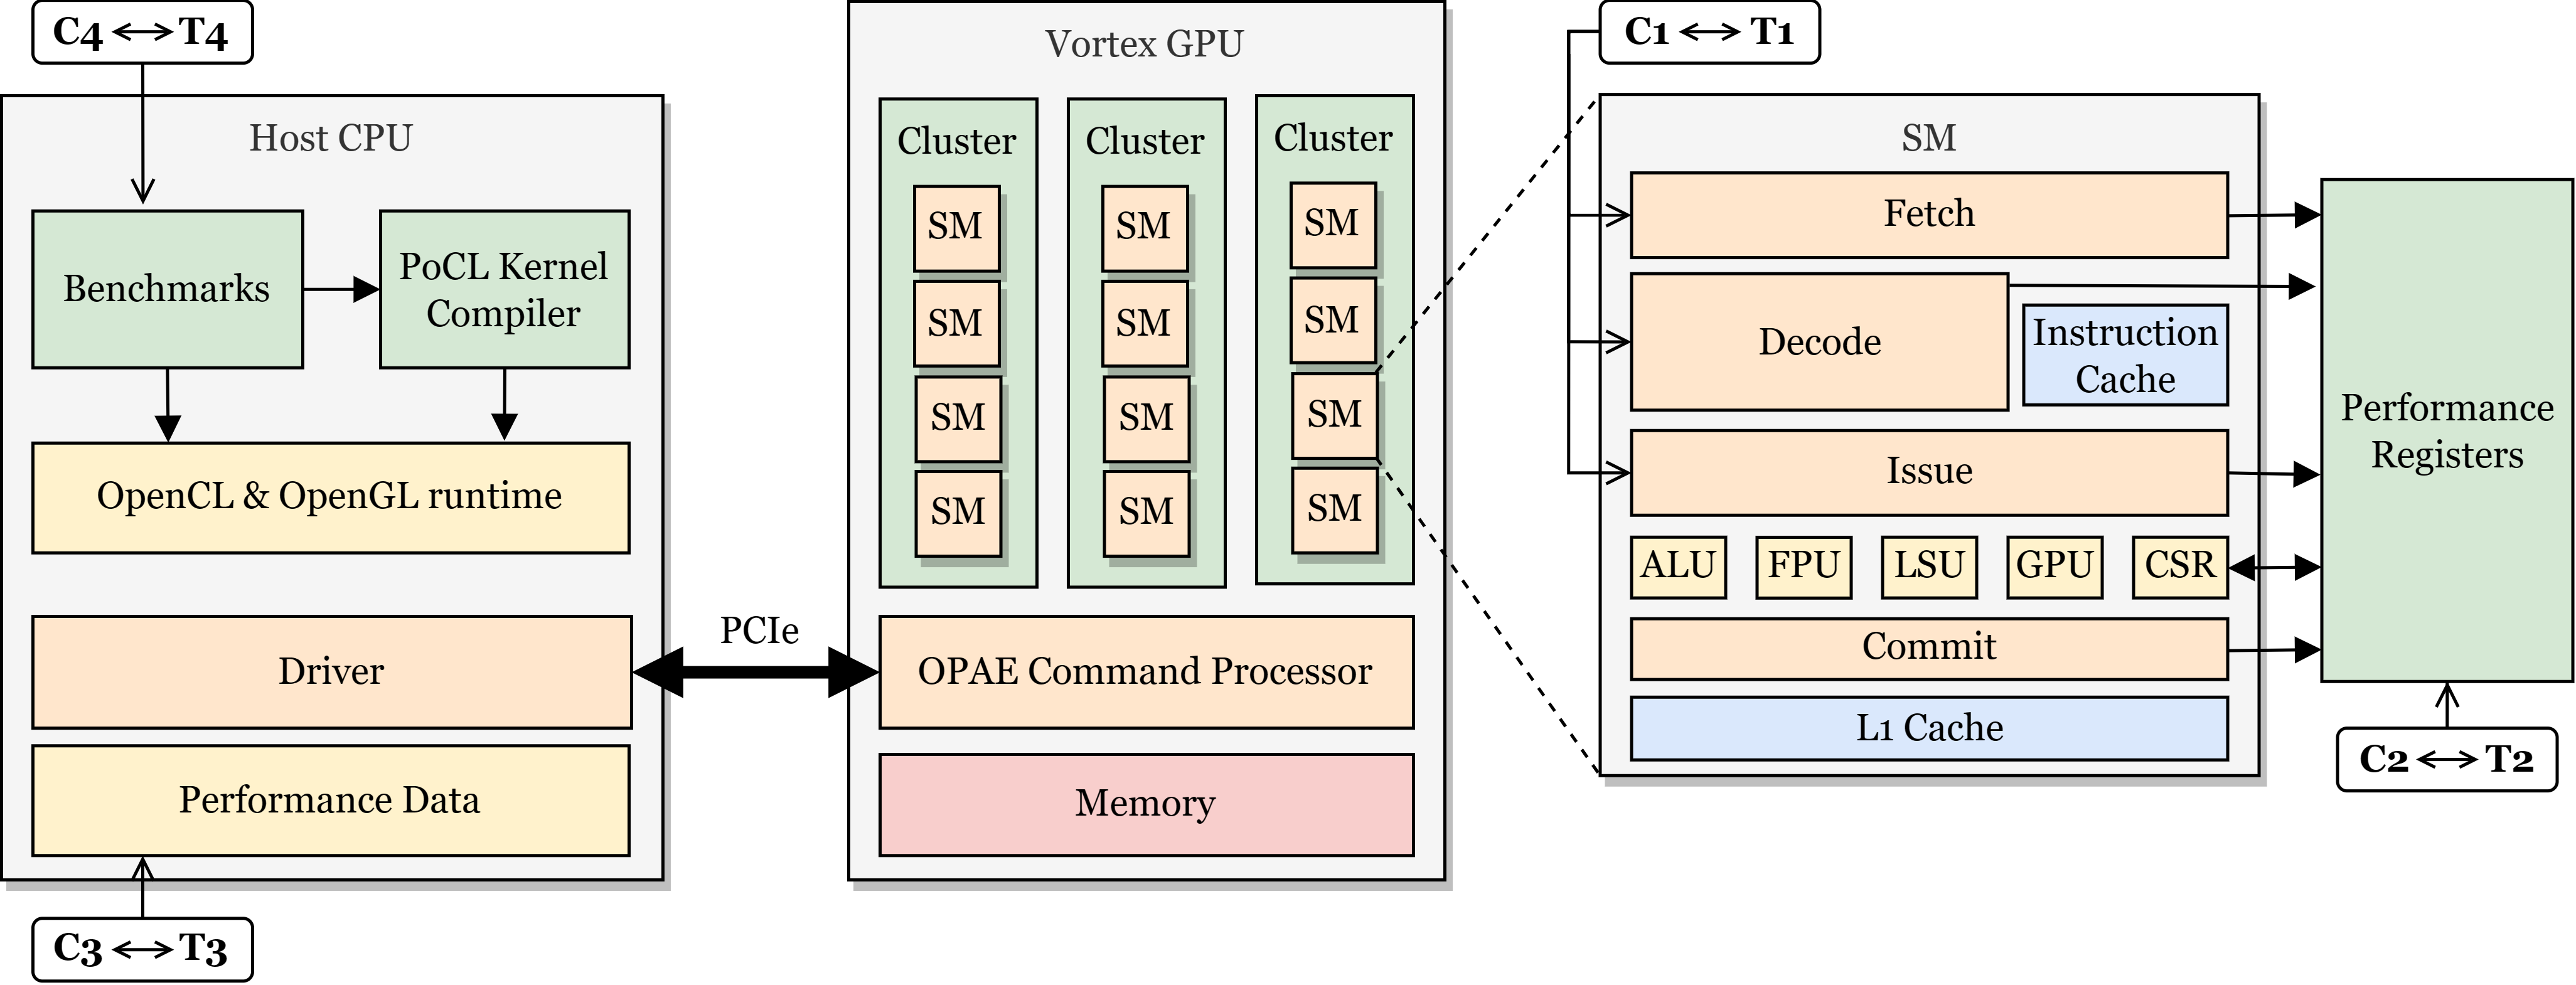
\includegraphics[width=\textwidth]{figures/task-contribution-4.png}
    \caption[High-level overview of the \Gls{vortex} \acrshort{gpu}]{High-level overview of the \Gls{vortex} \acrshort{gpu} based on \cite{vortex}. The overview also shows how the tasks and contributions relate, and where in the project the contributions are made.}
    \label{fig:task-contribution}
\end{figure}

\section{Assignment Interpretation} \label{sec:tasks}

In this thesis, I will continue the work done in my project thesis~\cite{Aurud_Project}. The \text{overarching} goal of the project- and master thesis is to aid the \Acrfull{cal} at NTNU to simulate and evaluate \acrshortpl{gpu} using \acrshortpl{fpga}. I define the following list of tasks based on my interpretation of \hyperref[chap:assignment]{the assignment text}:

\begin{itemize}
    \item[\textbf{T1}] Propose and implement a set of improvements to the \Gls{vortex} \acrshort{gpu} based on results and \acrshort{cpi} stacks obtained in my project thesis.
    \item[\textbf{T2}] Improve \acrshort{csv} to give a better overview of the issue stage. 
    \item[\textbf{T3}] Evaluate the implemented improvements.
    \item[\textbf{T4}] If time permits, evaluate the observed problems and proposed solutions using a commonly used GPU benchmarks suite such as Rodinia.
\end{itemize}

\newpage
Task \textbf{T2} was added during the development of the improvements, as I discovered that my existing version of \acrshort{csv} was too connected to \Gls{vortex}' issue scheduler. This blocked \acrshort{csv} from giving a good overview of the issue stage and stall causes.

\section{Contributions} \label{sec:contributions}

In this thesis, I make the following key contributions:
\begin{itemize}
    \item[\textbf{C1}] I propose and implement changes to \Gls{vortex}' fetch, decode and issue stage to increase fetch and issue bandwidth, solving the problems identified in my project thesis.
    \item[\textbf{C2}] I improve upon \acrshort{csv}, enabling it to identify the stall cause for all warps in the instruction buffer and attributing them accordingly.
    \item[\textbf{C3}] I evaluate the implemented improvements using \acrshort{cpi} stacks and other collected performance metrics. I find that the changes move the frontend bottleneck to the backend of the \Gls{gpu}, showing that \Gls{vortex} is unable to hide latency stalls.
    \item[\textbf{C4}] I expand \Gls{vortex}' benchmark suite by porting a majority of the \Gls{rodinia} benchmarks. Additionally, I improve core components of \Gls{vortex}' mechanisms to collect performance metrics, making it more accurate and allowing multi-kernel programs to be used for benchmarking.  
\end{itemize}

The tasks and contributions are linked one-to-one, i.e. $\textbf{Tx}\leftrightarrow~\textbf{Cx}$. Figure~\ref{fig:task-contribution} also describe how the tasks and contributions relate and where in the project the contributions are made.

\section{Outline}

Following is an outline of the rest of the thesis:

\begin{itemize}
    \item \textbf{Chapter 2} covers background information regarding GPUs, the GPU programming model and GPU simulation.
    \item \textbf{Chapter 3} first describe in detail the main components of \Gls{vortex}, and why the frontend is a bottleneck. Then it covers my proposed changes to solve the problems.
    \item \textbf{Chapter 4} contains details regarding how I ported a wide range of \Gls{rodinia} benchmarks to run on \Gls{vortex}.
    \item \textbf{Chapter 5} describes my methodology for collecting performance metrics to generate \acrshort{cpi} stacks.
    \item \textbf{Chapter 6} includes information regarding the experimental setup and \Gls{vortex} configuration.
    \item \textbf{Chapter 7} contains the results and evaluation of the proposed changes, in addition to a sensitivity analysis.
    \item \textbf{Chapter 8} contains the conclusion and thoughts regarding further work.
\end{itemize}

\begin{figure}
    \centering
    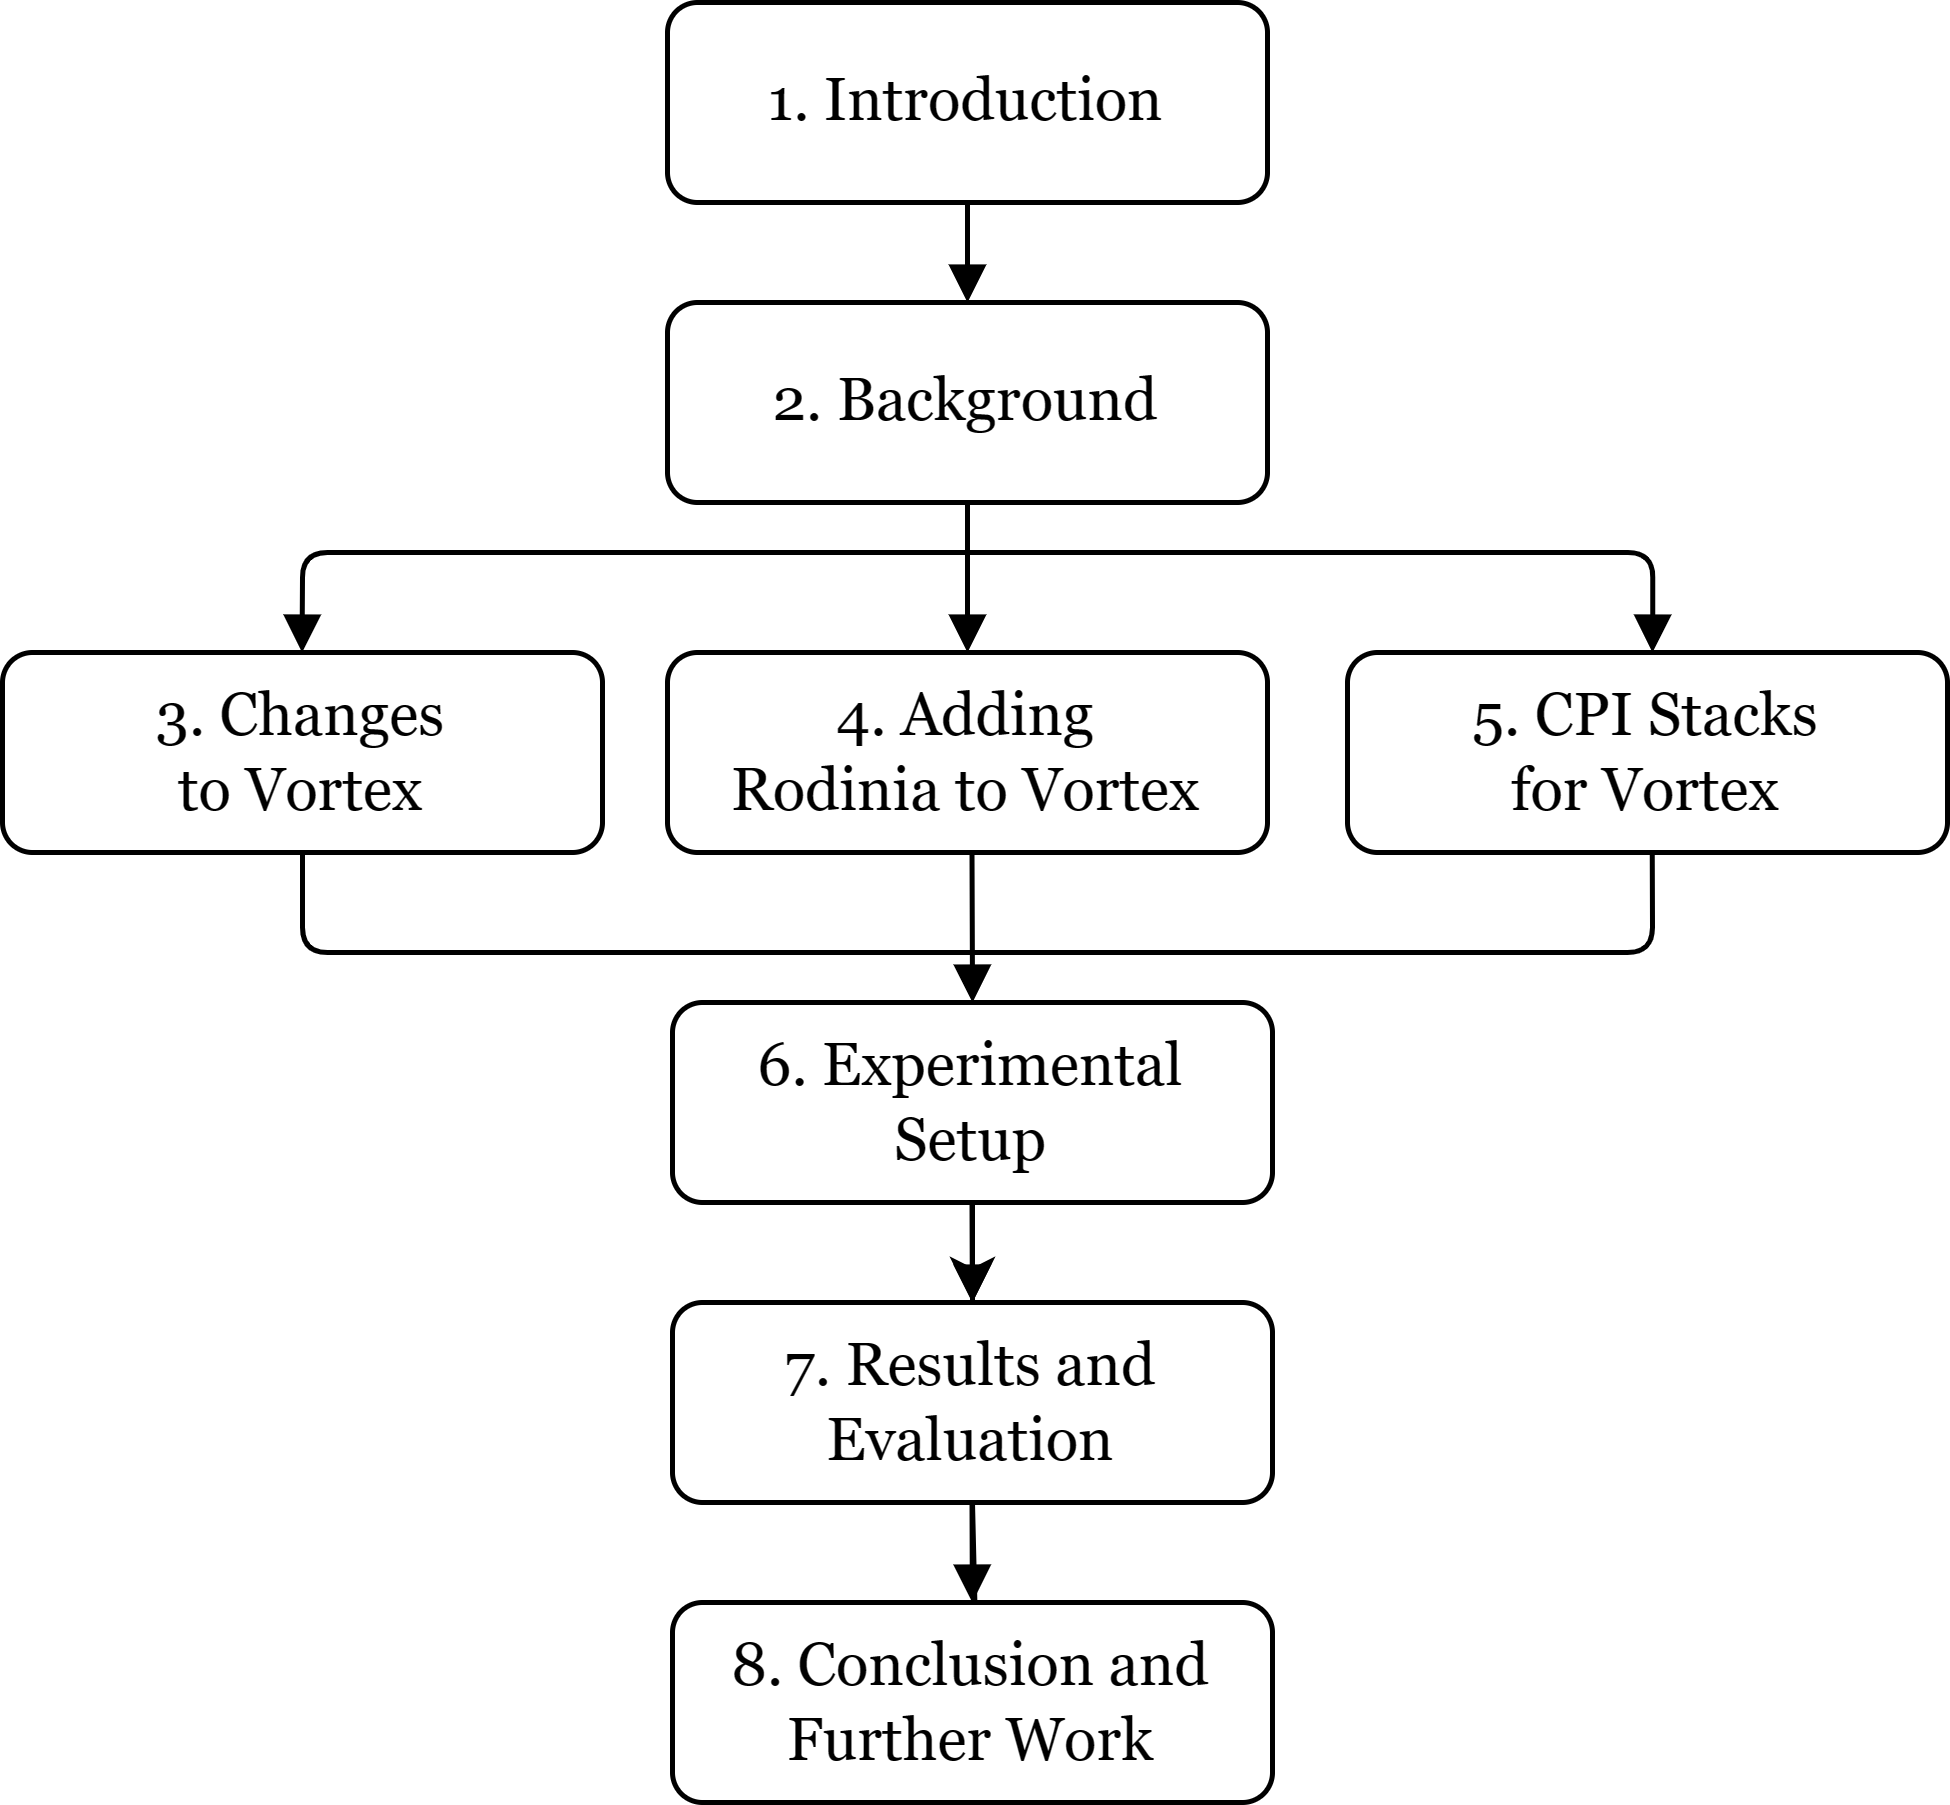
\includegraphics[width=0.8\textwidth]{figures/thesis-outline.png}
    \caption[Thesis outline]{Outline of the thesis. Chapter 3, 4, 5 and 7 contain the contributions made by me.}
    \label{fig:thesis_outline}
\end{figure}